We present an approach for automatically identifying the script of the text localized
on the scene images. Our approach is inspired by the advancements in mid-level features.
We represent the text images using mid-level strokes based features which are pooled from
densely computed local features. Once text images are represented using the proposed bag-of-strokes representation, we use an off-the-shelf classifier to identify the script of the text image. Our approach is efficient and requires very less labeled data. We evaluate the performance of our method on a recently introduced \textsc{cvsi} dataset, demonstrating that the proposed approach can correctly identify script of 96.70\% of the text images. In addition, we also introduce and benchmark a more challenging Indian language scene text dataset for evaluating the performance of
our method.
%\end{abstract}
%\begin{keywords}
%Bag of strokes, script identification, scene text
%\end{keywords}
\section{Introduction}
Reading text in scene images can provide useful information about the content
of the image. In multilingual country like India, sign boards often contain text of regional languages along with English and Hindi. The first step of reading text in such images is to answer ``what script is this?". The goal of this paper is to answer this question (see Figure~\ref{fig:firstRes}). To this end we use off-the-shelf text localization method and propose a novel mid-level feature based representation which we call bag-of-strokes, for robust script identification. The proposed method achieves an accuracy of 96.70\% on a recently introduced Video Script Identification (\textsc{cvsi}) dataset~\cite{CVSIComp}. For comprehensive evaluation of our method we also introduce and benchmark a more challenging 
Indian Language Scene Text (\textsc{ilst}) dataset in this work. The code and data used in this work will be made available on our project website\footnote{\url{http://cvit.iiit.ac.in/projects/SceneTextUnderstanding/}}.
 
Script identification in printed and handwritten document
images is a highly researched problem~\cite{GhoshDS10,scriptICDAR15,Pal}. Contrary to the scanned and handwritten images, script identification in scene images poses many additional challenges such as, (i) lack of context. Scene text often appears as a single word or a group of words, and applying larger sentence or paragraph level context is hard. (ii) stylish fonts. Scene text images often contains stylish fonts to attract the viewers and do not easily generalize to the training data, (iii) complex background. Scene text come with highly complex natural scene background, on the other hand document images often contain predominantly text. In case of scene images text localization and dealing with the false detection are few additional challenges. In this work we demonstrate the cropped word script identification as well as end-to-end script identification on scene images. To our knowledge end-to-end script identification on scene images have not been attempted in prior works.
\begin{figure} [!t]
\centering
\fbox{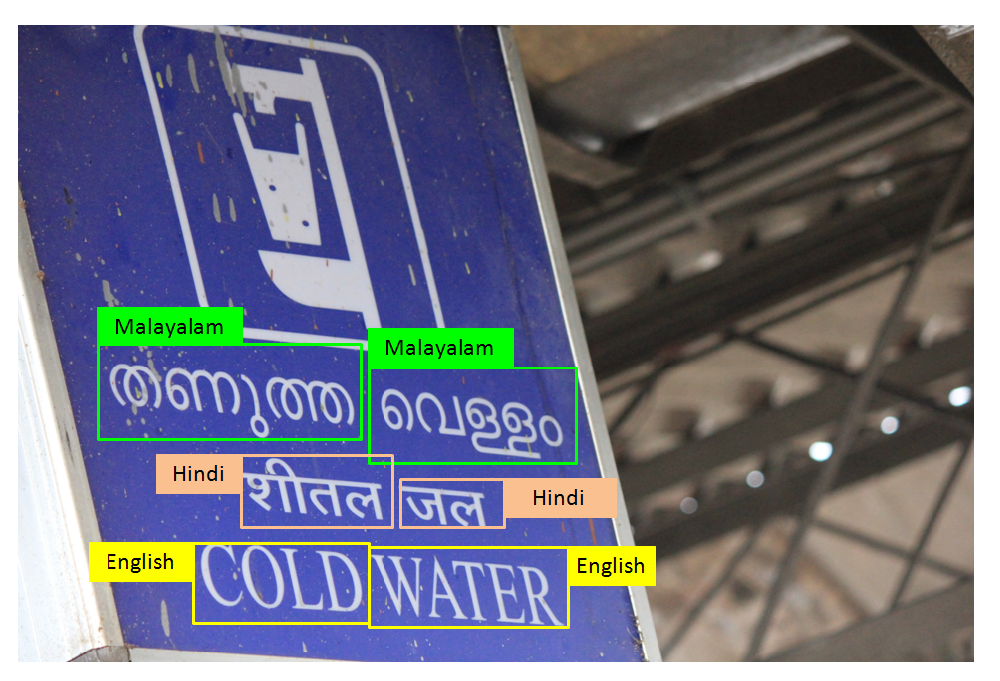
\includegraphics[width=.465\textwidth]{figures/Introduction.eps}}
\caption{A typical example of a street scene image captured in a multilingual country, e.g. India. Our goal in this paper is to localize the text and answer ``what script is this?" to facilitate the reading in scene images.}
\label{fig:firstRes}
\end{figure} 

There are many methods in the literature for script identification~\cite{CVSIComp,GhoshDS10,PhanSDLT11,JoshiGS07,Pati,SIWIcdar}
Texture based features such as Gabor filter~\cite{Pati}, \textsc{LBP}~\cite{LBPOjala2002} have been used for script identification. Joshi~\textit{et al.}~\cite{JoshiGS07} proposed multi-channel \textit{log}-Gabor filter bank and hierarchical classification scheme for script identification in Indic language documents. Reader is encouraged to refer~\cite{GhoshDS10} for detailed survey of classical methods in this area. 
These classical methods, though achieve high performance on printed documents, are not very successful in our case (see Section~\ref{sec:expts}). More recently in \textsc{icdar} 2015, competition for script identification on video text has been organized~\cite{CVSIComp}. We compare our method with the entries for this competition and show that our method is comparable to the top performing methods in this competition. There have been few contemporary methods based on deep learning~\cite{SIWIcdar,CVSIComp} and \textsc{rnn}~\cite{scriptICDAR15}. These methods achieve noticeable success on some of the selected benchmarks. However, these methods often require huge training data and computation resources.
 
In this paper, we propose a simple and effective solution for script identification in the wild. Our method is inspired by recent advancements made in mid-level features~\cite{FernandoFT14,JunejaVJZ13,BoureauBLP10}. First, we densely compute the local features on the given image and then pool these local features to encode the larger context about the given image. In our case, these larger context encode the strokes
of the scripts. We represent each training image using bag of these strokes and learn a classifier to identify the script of a test image. The advantages of our method are two fold, first, it is robust to variations and noise commonly present in the scene text. And second, the method is easily trainable and computationally efficient. 
\begin{figure*}[!t]
\centering 
\begin{subfigure}[]{
\includegraphics[width=5.5cm,height=5cm]{figures/Datasetfigures/figure1_1.jpg}
\includegraphics[width=5.5cm,height=5cm]{figures/Datasetfigures/figure2_2.jpg}
}
\end{subfigure}
\begin{subfigure}[]{
  \includegraphics[width=5.5cm,height=5cm]{figures/Datasetfigures/datasetCropped_1.png}
}  
\end{subfigure}
  \caption{Few example images from thee \textsc{ilst} datset we introduce. (a) we provide ground truth text bounding box, script and text for the images. (b) Few cropped word images of our dataset. The dataset can be used for variety of problems including recognition, text localization etc.}
  \label{fig:dataset}
\end{figure*}

The remainder of the paper is organized as follows. 
We discuss about datasets in Section~\ref{sec:datasets}. Here,
we introduce Indian language scene text dataset for the problem.
In Section~\ref{sec:ourApp}, mid-level features and novel bag-of-strokes based feature representation for text images is introduced. Section~\ref{sec:expts} gives details of the evaluation protocols, and performance measures used in this work. Experimental settings, results, discussions, and comparisons with various techniques are also provided  in this section, followed by conclusions.

\section{Datasets}
\label{sec:datasets}
\subsection{The ILST dataset}
Scene text understanding has gained huge attention in last decade, and several benchmark datasets were introduced~\cite{ICDARcomp11, MishraBMVC12}.
Most of these datasets are for scene text localization and recognition in English. There are also few datasets~\cite{SIWIcdar,CVSIComp} of multiple scripts e.g., east Asian languages or Indian language video text. In this work we introduce Indian Language Scene Text (\textsc{ilst} in short) dataset which is a comprehensive dataset for Indian language scene text containing six scripts commonly used in India, namely Telugu, Tamil, Malayalam, Kannada, Hindi and English. The dataset contains 500 scene images with more than 4000 words. It can be used for following tasks: text localization, recognition, script identification. In this work we use this dataset for two tasks- cropped word script identification and text localization with script identification (i.e., end-to-end pipeline).
\\
\


\noindent\textbf{Comparison with other related datasets}
To our knowledge \textsc{ilst} dataset is the largest scene text dataset for the Indian languages. Other related datasets such as \textsc{cvsi}~\cite{CVSIComp}, SIW~\cite{SIWIcdar} are only meant for script identification on cropped words whereas ours can be used for many other related tasks e.g., recognition and text localization. Also, the dataset is collected in a realistic setting and has wide variations in scale, font style, background and illumination. 
\\
\


\noindent\textbf{Mode of collection.} We have collected the images for this dataset by either capturing pictures in streets of various cities in India, harvesting images from Google image search or importing and providing annotation for few images from other existing datasets. These images contain signboards, billboards, posters mainly from urban part of the country. We have collected these images in an unconstrained manner, i.e., without considering much of the view angle. Further, various digital cameras with diverse camera settings were used while capturing images. These are intentionally done to create a realistic dataset.
\\
\


\noindent\textbf{Annotations.} 
For annotations of the scene images, we use a publicly available web based tool~\cite{labelme}. All the annotations are provided in XML for each image separately describing global image features, bounding boxes of text and its special characteristics. The XML-Schema of LabelMe has been adapted and extended by tags for additional metadata. 

Each text field (word) in the image is annotated with following attributes: (i) word bounding box. These bounding boxes are rectangular and parallel to the axes. (ii) ground truth text, (iii) the inherent script of the text, and additional information such as, (iii) illumination, (iv) blur, (v) occlusion, and (vi) 3D Effects. 
\\
\


\noindent\textbf{Train-Test splits.}
We provide a standard train and test splits for this dataset. We use randomly chosen 30\% images of the dataset for the training and the rest for testing. We will make this dataset publicly available on our project website. The details of dataset is provided in Table~\ref{tab:dataset}. We also show few example images of our dataset in Figure~\ref{fig:dataset}. 

%We intend to extend ILST dataset to 10 popular scripts used in India, and collect and annotate approximately 10K images in future.


%\begin{figure}[t]
%  \includegraphics[width=8cm]{figures/variationsWords_1.png}
%  \caption{Variations presents in different word images.}
%  \label{fig:variationWords}
%\end{figure}


%\subsection*{\textbf{Global Image Metadata}}
 
%\subsection*{\textbf{Textfield Metadata}}
%The All words in natural images of dataset are marked by bounding boxes. Bounding boxes are rectangular and parallel to the the axes. The metadata is enriched by some of the typographical and geometrical characteristics along with difficulty level for identification. The texfield metadata includes:
%
%\begin{enumerate}[(a)]
%
%	\item \textbf{Language:} Languages are very important information when we try to identify and recognize the words. There are five Indic Scripts which we are using for script identification.
%	\item \textbf{Illumination}
%	\item \textbf{Occlusion}
%	\item \textbf{Blurredness}
%	\item \textbf{3D Effects}
%
%\end{enumerate}

\begin{table}
%\begin{center}
\caption{The ILST dataset: we introduce a \textsc{ilst} dataset which contains 578 scene images and 4036 cropped images from 5 major Indian languages.}
\centering
\begin{tabular}{|l|c|c|c|}
\hline

Languages & $\#$ scene images & $\#$ word images & Mode of collection\\
\hline\hline
Hindi & 76 & 514 & Authors, Google Images \\%& Team Members \& Internet \\
\hline
Malayalam & 121 & 515 & Authors, Google Images  \\
\hline
Kannada & 115 & 534 & Char74K~\cite{deCampos09}\\
\hline
Tamil & 59 &563 & Authors \\%& \\
\hline
Telugu & 79 &510 & Authors \\%& \\
\hline
English & 128  & 850 & Authors \\%& \\
\hline
total & 578 & 4036 & -\\
\hline
%Total &\multicolumn{3}{c|}{2636} \\
%\hline 

\end{tabular}
\label{tab:dataset}
\end{table}

%\begin{figure*}[!t]
%\centering
%\subfigure{
%\label{fig:subfig3}[a]
%\includegraphics[scale=1]{figures/annotation.png}
%}
%\subfigure{
%\label{fig:subfig3}[b]
%\includegraphics[scale=0.6]{figures/croppedWordSample.png}
%}
%\caption{(a) We annotate text images of various Indian languages in our newly introduced dataset. The annotation provides: (i) Text bounding box, (ii) Script (iii) ... [Plz write] (b) Few sample cropped word images of Kannada, Hindi and Malayalam are shown. We observe a high variations in dataset in terms of skew angle, illumination, noise etc. Further it can be seen Indian languages scripts are very similar to each other, which makes script identification for Indian languages a challenging problem.}
%\label{fig:challenges1}
%\end{figure*}
\subsection{CVSI 2015~\cite{CVSIComp}}
To show the genarality of our method, we also evaluate our method on the dataset which has been introduced in Video Script Identification Competition held at \textsc{icdar 2015}.  
The dataset is composed of images from news videos of various Indian
languages. It contains 6412 training text images and 3207 testing text images from 10 different scripts
namely, English, Hindi, Bengali, Oriya, Gujarati, Punjabi, Kannada,
Tamil, Telugu and Arabic, commonly used in India.

\section{Methodology}
\label{sec:ourApp}
In this section we introduce our bag-of-strokes based representation of text images for script identification task. First, we briefly give motivation and overview of our method, compare it with closely related works, and then give the details of how we obtain bag-of-strokes representation by pooling local low level features. We finally summarize the full pipeline of our approach.

\subsection{Motivation and overview}
Mid-level feature representation have gained huge attention in last few years. These features are potentially more distinctive than the traditional low-level local features constructed in a purely bottom-up fashion~\cite{FernandoFT14}. Mid-level features have achieved noticeable success in image classification and retrieval tasks~\cite{JunejaVJZ13,BoureauBLP10,FernandoFT14}. Our method is inspired from these methods as we present a novel bag-of-strokes based features which are robust for the task of our interest, i.e., script identification in the wild. 

Script identification in the wild is a challenging problem. The traditional  low-level local features are not competent for this task. This is primarily due to the imaging, variation in scale, ambiguity, sharing of strokes in the scene text images. On the other hand strokes are the atomic units of scripts and collection of strokes are discriminative enough for the task of identifying the scripts (see figure~\ref{fig:strokes}). Our method is build on these intuitions. In this work, given a text image we first densely compute local visual features, and then pool these local features into frequently occurring larger patterns (or strokes) and each text image is represented using histogram of these larger patterns (or strokes). 
\\
\


\noindent\textbf{Comparison with other related approaches:} 
The mid-level features have outperformed the na\"{\i}ve bag-of-visual-words based features for image classification~\cite{JunejaVJZ13}, because of their
robustness and better discriminating power. Usually these mid-level
features capture the larger context in the image as compared to the local or semi-local features. One alternative to use larger context is to simply cluster larger patches, as done for local feature computation. However such method are not effective in our case due to the large variability in scene text images. In context of supervision methods, mid-level features can
be grouped into three categories: supervised~\cite{JunejaVJZ13}, weakly-supervised~\cite{FernandoFT14} and unsupervised~\cite{SinghGE12}. Our method falls in weakly supervised category where we only need the class information. 

\begin{figure} [!t]
\centering
\fbox{\includegraphics[scale=1.1]{figures/strokes.png}}
\caption{Strokes are atomic units of scripts. We show some representative strokes of following scripts (top to bottom): Hindi, Kannada, Malayalam, Tamil and Telugu. Our method yields the strokes which are representative and discriminative enough for a cropped image.}
\label{fig:strokes}
\end{figure} 

\begin{figure*} [!t]
\centering
\fbox{\includegraphics[scale=0.7]{figures/pipeline.jpg}}
\caption{Method Overview: The figure depicts the feature computation process where, first we find the local features from the images, we cluster these feature to get the local histogram of visual words. Then we cluster the histogram of visual words to get the representation of words in form of strokes.}
\label{fig:overview}
\end{figure*} 

\subsection{Bag-of-strokes based representation}
\label{sec:bos}
We compute the bag-of-strokes representation of words from a labeled data. The  overview of our method is illustrated in Figure~\ref{fig:overview}. Given training text image $I_i$ and its script $s_j$ where $s_j \in {\cal S}$ (set of scripts), we follow the following steps.
\begin{itemize}
\item First, we densely compute the local features and represent each training image $I_i$ 
as a set of descriptors (see Section~\ref{sec:features} for details of feature computation).
\item All the descriptors are then clustered to obtain visual words. Let $C = \{c_1,c_2,...,c_m\}$ be the set of visual words with vocabulary size = $m$. 
\item We obtain assignment for every feature $\phi_k$, i.e., obtain the feature-visual word pair $(\phi_k, c_l)$
\item In a $p \times q$ rectangular neighborhood around feature $\phi_k$ we obtain a local histogram of visual words $H_k$. These $H_k$s capture a larger context and are
more discriminative patterns. Indeed they are strokes in our case. 
\item We again cluster local histograms $H_k$ to obtain larger patterns which encode the
strokes. Let $\psi = \{\psi_1, \psi_2, \cdots ,\psi_n\}$ be the set of such clusters with stroke vocabulary size = $n$.
\item Once $H_k$ and $\psi$ in hand, we assign every local histogram $H_k$ to one of cluster from $\psi$. In other words, each image is represented as bag of strokes. We
name this representation $\chi$.
\end{itemize}  
At the end of this process each word image in the training data is represented with bag-of-strokes $\chi$. To only use the best strokes we prune few less informative strokes by using the method described in Section~\ref{sec:best}.

\subsubsection{Feature computation}
\label{sec:features}
%Given a set of word images from Indic scripts scene text
%$R = (\{I_i, Z_i\})_{i=1}^n$, where $I_i$ is an image and $Z_i$ is the script label of the word image. The goal of our method is to learn a set of distinctive strokes from $R$. These strokes should be able to capture the essential distinctive parts from the image, which then be used to classify the different scripts for given words. The $R$ contains the training images, which will be used for discovery of discriminative strokes. 

%These strokes can be found by using the unsupervised Elkan variant of K-means algorithm, since it learns both discriminative and representative strokes from the word images.

Given a text image we compute the SIFT descriptors at points on a regular grid with spacing of $M$ pixels. At each point the descriptors are computed over four circular support patches with different radii, consequently each point is represented by four SIFT descriptors. We also learn the multiple descriptors to allow the scale variation between images. At each grid point the descriptors are computed over circular support patches with radii $r = 4,6,8$ and $10$.

%After the descriptors have been computed, the vocabulary of strokes are learned in offline unsupervised manner. The descriptors computed above are clustered using Elkan variant of $K$-means algorithm. The cluster initialization is done by using $K$-means++ which greedily picks $k$ data points that are maximally different, here $k=4000$. After the vocabulary has been created, every word image is represented with the help of histograms of the strokes in vocabulary as $[h_1, \ldots, h_k]$ where $h_i$ is the number of occurrences of the $i^{th}$ stroke in the image. To incorporate the spatial information, the Spatial Pyramid Strategy \cite{Lazebnik} ($2\times4$ grid) is also used.
\subsubsection{Finding the best strokes for the task}
\label{sec:best}
We wish to use the bag-of-strokes $\chi$ as a novel set of mid-level
features to describe the text image. But not all strokes are
are relevant for the task of script identification, e.g., 
a stroke commonly occurring in all the scripts may not carry
useful information (not~\emph{discriminative}). Moreover, there 
are few strokes which can occur in most of the images in a script 
and are very good~\emph{representative} of that script. To measure
discriminativity and representativity of a stroke $str \in \chi$  we compute following relevance score:
\begin{equation}
rel(str) = D(str) \times R(str),
\end{equation}
where $D(str)$ and $R(str)$ are discriminativity and representativity scores respectively. To compute $D(str)$ and $R(str)$ we follow entropy based formula.
We compute the entropy of stroke by considering (i) scripts as class (script specific entropy) (ii) individual images in scripts as class (image specific entropy). We use these entropies to define $D(str)$ and $R(str)$ such that lower value for script specific entropy and higher value for image specific entropy results in higher values of $D(str)$ and $R(str)$. This ensures that those strokes which are found in certain script and almost all the images of that script are more relevant. We prune the bottom 20\% less relevant strokes before representing images using bag-of-strokes. 

\begin{table}[!t]
\caption{Results on ILST (cropped words script identification)} 
\centering
\renewcommand{\arraystretch}{1.5}
\begin{tabular}{|l|c|}
  \hline              
  \textbf{Method} &~\emph{\textbf{Accuracy} (\%)}   \\      
  \hline\hline
\textit{Baseline Methods} & \\
~~~Gabor features~\cite{Pati} & 59.25 \\ 
~~~Gradient features & 47.74 \\ 
~~~Profile Features~\cite{Manmatha12} & 49.24 \\
~~~LBP~\cite{LBPOjala2002} & 78.08\\
\hline\hline
\textbf{Ours} & \textbf{88.67} \\
  \hline  
\end{tabular}
\label{tab:ILSTRes1} 
\end{table}

\subsection{Script identification: Full pipeline}
Given a scene image our goal is to localize text and then identify its script.
To this end we first obtain text localization using a method proposed in~\cite{GomezK14}
and an open source OCR~\cite{tessOCR}. While the text localization technique we apply is rather standard, we adapt this for the multi-script dataset we use. 
Once the text is localized we represent it using bag-of-strokes representation which is learned from the training data (discussed in Section~\ref{sec:bos}). Each localized
text is now fed to a linear SVM classifier which is trained for the task to obtain the inherent script.

\section{Experiments}
\label{sec:expts}
Given a scene image containing text our goal is to localize the text and identify it's script. We show results in two settings, (i) end-to-end pipeline, and (ii) cropped word script identification on the datasets presented in Section~\ref{sec:datasets}.
In this section we provide details of implementation, evaluation protocols and baseline methods, and evaluate the performance of our method and compare it with previously published works.

%\begin{table}[!t]
%\caption{Results on ILST (cropped words script identification)} 
%\centering
%\begin{tabular}{lc}
%  \hline              
%  Method &~\emph{Accuracy (\%)}   \\      
%  \hline
%\textit{Baseline Methods} & \\
%~~~Gabor features & \\
%~~~LBP & \\
%~~~Moment features & \\
%Ours & \\
%  \hline  
%\end{tabular}
%\label{tab:ILSTRes1} 
%\end{table}
%\begin{table}[!t]
%\caption{Results on CVSI. We compare our method with the top-performing
%methods in the ICDAR 2015 competition} 
%\centering
%\begin{tabular}{lc}
%  \hline              
%  Method &~\emph{Accuracy (\%)}   \\      
%  \hline
%\textit{Competition entries} & \\
%~~~C-DAC & \\
%~~~CVC-1 & \\
%~~~CVC-2 & \\
%~~~HUST & \\
%~~~Google & \\
%Ours & \\
%  \hline  
%\end{tabular}
%\label{tab:CVSIRes1} 
%\end{table}

\begin{table}[!t]
\caption{Results on ILST (End-to-End pipeline). We use~\cite{GomezK14} and tesseract~\cite{tessOCR} for text localization and evaluate our proposed method of script identification based on measure presented in Section~\ref{sec:perf}} 
\centering
\begin{tabular}{|l|c|c|c|}
  \hline    
  Script &~\emph{Precision}&~\emph{recall}&~\emph{f-score}  \\      
  \hline\hline          
  Telugu & 0.47 & 0.54 & 0.51 \\
  Tamil & 0.41 & 0.44 & 0.42\\
  Malayalam & 0.49 & 0.45 & 0.47 \\
  Kannada & 0.39 & 0.47 & 0.42\\
  Hindi & 0.42 & 0.48 & 0.45\\
  English & 0.46 & 0.56 & 0.50\\
  \hline  
\end{tabular}
\label{tab:ILSTRes2} 
\end{table}

\subsection{Implementation details and design choice}
The proposed method is implemented on a system with 16 \textsc{gb ram} and
Intel${^\noit\textregistered}$ Core$^{\noit{\textsc{\scriptsize{tm}}}}$ \textit{i3-$2105$} \textsc{cpu} $@$ 3.10GHz system. The proposed system takes approximately \textbf{0.4 \textit{millisecond}} to identify the script of a cropped word. The two important parameters visual word vocabulary size $m$ and stroke vocabulary size $n$ (refer Section~\ref{sec:bos}) were empirically chosen as 4K and 3K respectively. The parameter C in SVM is obtained using grid search on independent validation set. We keep these parameters fixed for all our experiments.  

\subsection{Evaluation Protocols}
\label{sec:perf}
\noindent \textbf{End-to-end script identification.}
We evaluate our method on end-to-end pipeline of script
identification. For this we first localize the text 
in scene images. We use a standard available text localization
scheme for localizing the text. Obviously, this step misses 
some text regions and produces few false bounding boxes. 
We fed all the text candidate bounding boxes to script identifier.

It should be noted that end-to-end script
identification is far more challenging than
script identification in cropped words or
document images. Since the final score of
this reflects the error accumulated due to text localization
and incorrect script identification.

To evaluate the end-to-end script identification
we use standard measures, precision ($prec$),
recall($rec$) and $fscore$ computed for every script.
For every script $s$ we compute following terms: 
(i) number of correctly identified words ($TP_s$). A detected word
is called correctly identified if the intersection
by union overlap with the ground truth bounding box is more than 60\%
and it has the same script identified as the ground truth,
(ii) total number of identified words ($TI_s$), and
(iii) total number of ground truth words ($TG_s$)
 
Once these in hand we compute \textit{precision}, \textit{recall} and \textit{f-score}
for every script and every image. We then report mean of
these score over all the images in the dataset.  
\begin{equation}
prec_s = \frac{TP_s}{TI_s}
\end{equation}
\begin{equation}
rec_s = \frac{TP_s}{TG_s}
\end{equation}
\begin{equation}
fscore_s= 2~\frac{prec \times rec}{prec+rec}
\end{equation}
The ideal script identifier should achieve
$1$ for these measures for all the scripts.
\begin{figure}[t]
  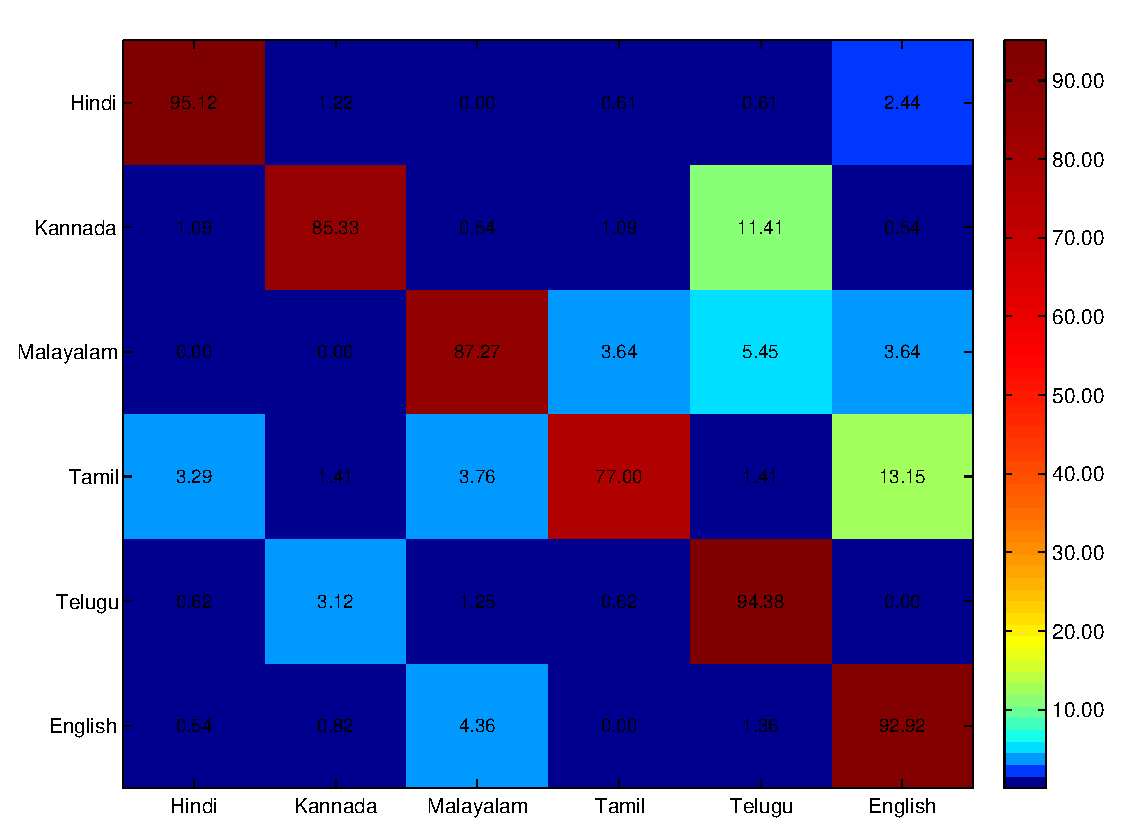
\includegraphics[scale=0.5]{figures/confusion_1.eps}
  \caption{Confusion matrix on ILST cropped words. Our method achieve a 88.67\% accuracy of script identification on the introduced dataset.}
  \label{fig:cm}
\end{figure}

\noindent \textbf{Cropped word script identification.}
We also evaluate our method on cropped words. For this we compute
accuracy which defined as follows:
\begin{equation}
Accuracy = \frac{{correctly~identified~words}}{{total~number~of~words}} \times 100.
\end{equation}
Here a word is called correctly identified if the method identifies script same as the ground truth.

\begin{figure}[t!]
\centering
\renewcommand{\arraystretch}{2.1}
\begin{tabular}{|l||ccc||c|}
\hline
\textbf{Language} & \multicolumn{3}{c||}{\textbf{Success}} & \multicolumn{1}{c|}{\textbf{Failure}} \\
\hline\hline
Hindi & \includegraphics[height=0.5cm,width=1.0cm]{figures/Results/Success/Hindi_4.jpg} & \includegraphics[height=0.5cm,width=1.0cm]{figures/Results/Success/Hindi_5.jpg} & \includegraphics[height=0.5cm,width=1.0cm]{figures/Results/Success/Hindi_6.jpg} & \includegraphics[height=0.5cm,width=1cm]{figures/Results/Failure/eng_tam.png} \\
Kannada & \includegraphics[height=0.5cm,width=1.0cm]{figures/Results/Success/Kannada_2.png} & \includegraphics[height=0.5cm,width=1.0cm,width=1cm]{figures/Results/Success/Kannada_3.png} & \includegraphics[height=0.5cm,width=1.0cm]{figures/Results/Success/Kannada_4.png} & \includegraphics[height=0.5cm,width=1.0cm]{figures/Results/Failure/Kannada-Telugu_4.png} \\
Malayalam & \includegraphics[height=0.5cm,width=1.0cm]{figures/Results/Success/Malayalam_1.jpg} & \includegraphics[height=0.5cm,width=1.0cm]{figures/Results/Success/Malayalam_2.jpg} & \includegraphics[height=0.5cm,width=1.0cm]{figures/Results/Success/Malayalam_3.jpg} & \includegraphics[height=0.5cm,width=1.0cm]{figures/Results/Failure/mal_tam.png} \\
Tamil & \includegraphics[height=0.5cm,width=1.0cm]{figures/Results/Success/Tamil_3.jpg} & \includegraphics[height=0.5cm,width=1.0cm]{figures/Results/Success/Tamil_5.jpg} & \includegraphics[height=0.5cm,width=1.0cm]{figures/Results/Success/Tamil_1.jpg} & \includegraphics[height=0.5cm,width=1.0cm]{figures/Results/Failure/tam_mal.png} \\
Telugu & \includegraphics[height=0.5cm,width=1.0cm]{figures/Results/Success/Telugu_1.png} & \includegraphics[height=0.5cm,width=1.0cm]{figures/Results/Success/Telugu_2.png} & \includegraphics[height=0.5cm,width=1.0cm]{figures/Results/Success/Telugu_3.png} & \includegraphics[height=0.5cm,width=1.0cm]{figures/Results/Failure/telugu_kan_1.png} \\
English & \includegraphics[height=0.5cm,width=1.0cm]{figures/Results/Success/English_1.jpg} & \includegraphics[height=0.5cm,width=1.0cm]{figures/Results/Success/English_2.jpg} & \includegraphics[height=0.5cm,width=1.0cm]{figures/Results/Success/English_3.jpg} & \includegraphics[height=0.5cm,width=1.0cm]{figures/Results/Failure/eng_kan.png} \\
\hline

\end{tabular}
\caption{Success and Failure Cases. Despite high variations in the dataset, our method correctly identifies the script of scene text images. The ``Success" columns depicts the correctly classified word images, and wrongly classified words are shown in ``Failure" column along with recognized script in red boxes.}
  \label{fig:visRes1}
\end{figure}

\subsection{Baseline Methods}
We compare our methods with popular features used for script identifications in document images
namely LBP~\cite{LBPOjala2002}, Gabor features~\cite{Pati}. We also evaluate gradient based features and profile features~\cite{Manmatha12} for script identification task and compare with our method. For comparison in CVSI dataset we compare our method with the best performing methods reported in~\cite{CVSIComp}.

%\noindent\textbf{Local Binary Pattern}  (\textsc{LBP})~\citep{} is a local descriptor that captures the appearance of an image in small neighborhood around a pixel. We compute the histogram of quantized \textsc{LBP} features per cell of size $16$.	

%\noindent\textbf{Profile Features}~\citep{ProfFeatPK2014} are used to represent the word images as a feature sequence. We calculate the features on a sliding window of size $20$ pixels with $75\%$ overlap. Features are then normalized with respect to the height of the word image.
%
%\noindent\textbf{Gabor Features}~\citep{ProfFeatPK2014} are computed by filtering the word images using the real parts of various different Gabor filter kernels. The energy of the filtered images are then used as features for classification. We used three different radial frequencies ($0.125$, $0.25$, $0.5$) and six angles of orientation ($\theta$) ($ 0 \degree$, $30 \degree$, $60 \degree$, $90\degree$, $120\degree$ and $150\degree$). The three radial frequencies with six $\theta$s give a combination of $18$ odd and $18$ even filters. And all the word images are filtered with these $36$ filters giving a $36$ dimensional gabor features.  

%\noindent\textbf{Gradient Features} ~\citep{Vibhor13} We used vertical strips of width $4$ pixels and a $2$-pixel horizontal shift to extract the histogram of gradient orientation features. We computed signed gradient orientation
%in this step. Each vertical strip was represented with a
%histogram of $9$ bins.
\begin{table}[!t]
\renewcommand{\arraystretch}{1.2}
\centering
\caption{Task specific evaluation on \textsc{cvsi}~\cite{CVSIComp}. Here A: Arabic, B: Bengali. E: English, H: Hindi,G: Gujrati, K: Kannada, O: Oriya, P: Punjabi, Ta: Tamil, Te: Telugu. Hence AEH means where
script identification of three class namely, Arabic, English and Hindi, is performed and so on. Further, Task-1, Task-2, Task-3 and Task-4 indicates tri-script, north Indian script, south Indian script, all script identification, respectively.}
\label{tab:CVSIRes2}
\begin{tabular}{|l|c|c|c|c|c|c|c|}
\hline
\multirow{2}{*}{Task} & \multicolumn{7}{ |c| }{Methods}\\
\cline{2-8}
& C-DAC & CUK & HUST & CVC-1 & CVC-2 & Google & \textbf{Ours}\\
\hline\hline
Task-1 & &  & & & & &\\
~~AEH & 95.46 & - & 99.79 & 97.32 & 96.80 & 100.00 & 100.00 \\
~~BEH & 91.40 & - & 98.36  & 94.68 & 94.27 & 99.49 & 98.61 \\
~~GEH & 88.33 & - & 99.09 & 96.38 & 95.98 & 99.4  & 99.41\\
~~KEH & 91.44 & - & 99.80 & 95.51 & 95.92 & 99.59 & 99.19\\
~~OEH & 95.87 & - & 99.50 & 96.88 & 96.37 & 99.19 & 99.49\\
~~PEH & 84.94 & - & 98.68 & 94.20 & 95.32 & 99.49 & 99.37\\
~~TaEH& 92.71 & - & 99.39 & 95.95 &  96.66 & 99.70 & 99.61\\
~~TeEH& 93.84 & - & 97.98 & 96.46 & 95.96 & 99.19 & 97.06\\
\hline\hline
Task-2 & 96.79 & 79.50  & 97.69 & 95.73 & 95.91 & 99.19 & 97.99\\
\hline\hline
Task-3 & 86.95  & 79.14 & 97.53 & 95.38 & 95.75 & 98.95 & 96.11\\
\hline\hline
Task-4 & 84.66 & 74.06 & 96.69 & 95.88 & 96.00 & 98.91 & 96.70\\
\hline
\end{tabular}
\end{table}
\subsection{Results on the ILST dataset}
\subsubsection{End-to-end script identification}
We evaluate end-to-end script identification on ILST dataset. To this end we first use public implementation of~\cite{GomezK14} for text extraction and then fed it to an open source OCR~\cite{tessOCR} to obtain text boundaries. Once we get bounding boxes we perform script identification using our method and evaluate performance based on performance measures presented in Section~\ref{sec:perf}. We summarize results of full pipeline in Table~\ref{tab:ILSTRes2}. We observe that our method achieves reasonably high~\emph{fscore} for this challenging task. The robustness of mid-level features we use can be attributed as factor for this success. It should be noted that text localization
is still an open problem and its performance affects the overall score of end-to-end script identification.  
\\
\


\subsubsection{Cropped word Script Identification}
We also show results on cropped words on \textsc{ilst} dataset. These results
are summarized in Table~\ref{tab:ILSTRes1}. Despite many challenges 
in this dataset (see figure~\ref{fig:dataset}) our method achieves 
script identification accuracy of 88.67\% which is significantly 
better than methods used in document image script identification domain such as~\cite{Pati,LBPOjala2002}.  To study script wise confusion we illustrate confusion matrix of our method for ILST dataset in Figure~\ref{fig:cm}.

\subsection{Results on CVSI dataset}
Following the protocols of \textsc{icdar} competition on video script identification~\cite{CVSIComp} we evaluate our method
following for four tasks: (i) Task-1: tri script identification
(ii) Task-2: north Indian script identification (iii) Task-3:
south Indian script identification, and (iv) Task-4: script identification
in all the ten scripts. 

We compare our method with top performing methods in this competition.
These results are summarized in Table~\ref{tab:CVSIRes2}. Our method
achieves 96.70\% for Task-4, i.e., script identification in all the ten
scripts and clearly outperform two methods in the competition namely, \textsc{C-DAC}
and \textsc{CUK}. Moreover, our results are marginally superior to \textsc{HUST}, \textsc{CVC-1},
\textsc{CVC-2} and comparable to the deep learning based best performing method
by Google.

\subsection{Qualitative evaluation}
We qualitatively evaluated our method in Figure~\ref{fig:visRes1} and Figure~\ref{fig:visRes2}. We show results on end-to-end as well as cropped word
script identification. We observe that despite high variations in images such as complex background, illumination change, low resolution our method is successful. Success and failure cases on the cropped image for six script are shown In Figure~\ref{fig:visRes1}. In failure section, Kannada text is wrongly classified as Telugu due to similarity in inherent scripts of both the languages. Similarly, Malayalam text is wrongly classified as Tamil and vice versa. These scripts are visually very similar and often challenges script identifier. It is also very interesting that, an English word is classified as Kannada due to the writing style. Adding location information (i.e., where the image is captured), context (i.e., scripts of neighboring text) can help mitigating such errors. We plan to add such features in our method in future.
\begin{figure}[t!]
\centering
  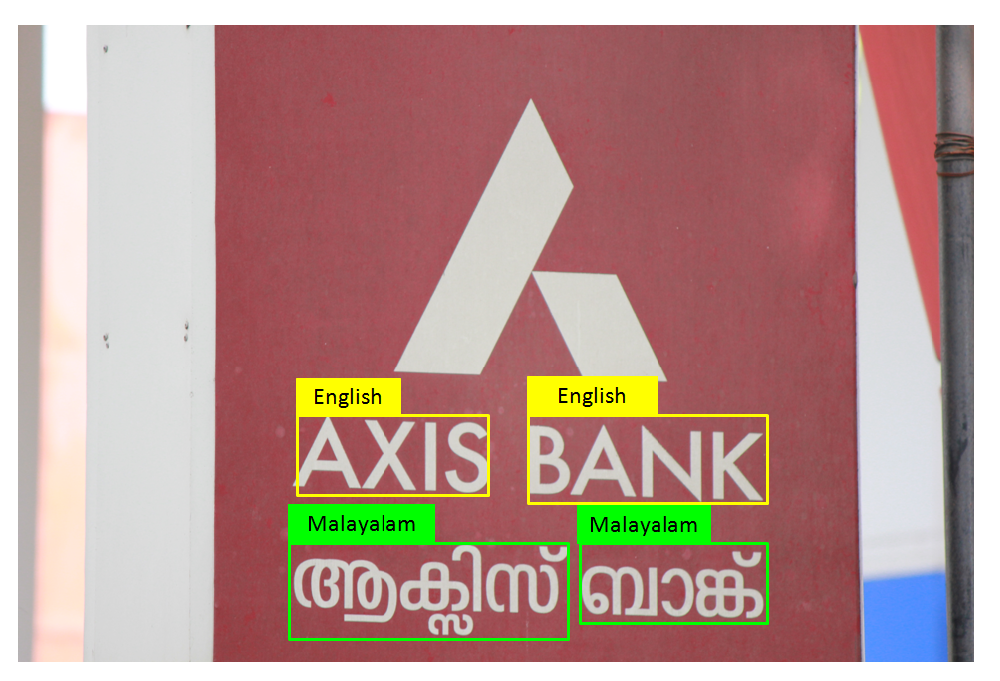
\includegraphics[scale=0.5]{figures/endtoend.eps}
 % \includegraphics[width=16cm]{figures/images.jpg}
  \caption{An example result of End-to-end script identification of our method. We localize the text boxes in images using method using~\cite{GomezK14} and~\cite{tessOCR}. Then we apply our method to find the inherent script in the text boxes.}
  \label{fig:visRes2}
\end{figure}
\section{Conclusions}
In this paper, we have addressed the problem of script identification in the wild. To this end we made following two important contributions: (i) we introduced a comprehensive dataset for Indian language scene text. This dataset will be useful for the community 
for many scene text related tasks in multilingual environment in the future. (ii) We have established a baseline for the end-to-end script identification pipeline for scene text and shown that simple mid-level features can achieve reasonably high performance for this task. As a future work we intend to extend our ILST dataset to 10 popular scripts used in India and explore the usage of multiple cues as aid to our script identifier, such as location of the image and neighboring texts. 

\label{sec:con}
